\documentclass[12pt,a4paper]{article}

\usepackage[a4paper,text={16.5cm,25.2cm},centering]{geometry}
\usepackage{lmodern}
\usepackage{amssymb,amsmath}
\usepackage{graphicx}
% \usepackage{svg}
% \svgsetup{inkscapelatex=false}
\usepackage{microtype}
\usepackage{hyperref}
\setlength{\parindent}{0pt}
\setlength{\parskip}{1.2ex}

\usepackage{placeins}

\let\Oldsection\section
\renewcommand{\section}{\FloatBarrier\Oldsection}

\let\Oldsubsection\subsection
\renewcommand{\subsection}{\FloatBarrier\Oldsubsection}

\usepackage{float}
\floatplacement{figure}{h!}

\usepackage[defaultlines=3,all]{nowidow}

\title{PeaceVote}

\author{Janis Erdmanis}

\usepackage[T1]{fontenc}
\usepackage{textcomp}
\usepackage{upquote}
%\usepackage{listings}

\usepackage{jlcode}

\renewcommand{\texttt}[1]{\jlinl{#1}}

\let\verbatim\trash
\lstnewenvironment{verbatim}
{}{}

\let\oldincludegraphics\includegraphics
\renewcommand{\includegraphics}[1]{\oldincludegraphics[width=0.5\textwidth]{#1}}


\begin{document}

\maketitle

% \abstract{PeaceVote abstract}

\section{Abstract}
The electronic voting problem had been studied extensively for decades, but still, the regular paper ballot currently is the only design capable of combining privacy with strong software-independence. I discuss that all electronic voting systems are doomed because authentification and mixnet cascades in curretn designs must be held by the same authorithy (must be trusted to some level) to avoid absence of election results. This constraint lead to dystopian designs where we are obligated to trust authority in production of ellection results which is a biological machine running software itself. To come around authentification pit hole, I propose braiding as a method to generate anonymous pseudonyms on absolute consent basis of each participant. I demonstrate how braiding can also be used to form immutable ledger BraidChain and how all those elements come together in the PeaceVote protocol where all trust in the authority had been decentralized to the trust of the software running on the devices. Lastly, I will cover network infrastructure, infiltrator and secrecy attacks and how those are resolved.\par
\section{Introduction}
In a regular paper ballot, everyone can see that officials are acting according to agreed and fair rules and are also able to take part without particular expert knowledge. On the contrary electronic voting schemes suffer from lack of openness and transparency, leaving doubt on whether the election officials are running the software that they claim to do and are not producing fake proofs to support their claims. That made Ron Rivest introduce a term software independence - a software is said to be software independent if election outcome is independent of undetected modifications to the software which runs the elections.\par
It is rather easy to design an electronic voting system which is software-independent but does not preserve privacy. In a simple design, each citizen would own state-certified public/private key pair which forms a digital identity of the person. To run the elections, the state would publish possible option messages. It would collect option certificates (signed documents) from the voters and publish them to for everyone accessible bulletin board for everyone to validate and count them.\par
Preserving voters privacy in an software-independent system is hard, and all known systems make compromises. There are two issues with combining software independence and privacy. To achieve software independence, the data making a conclusive proof for accounting components of the system must be collected and published. This data shall contain votes for everyone with cryptographical links proving that it was produced during the elections by a legitimate voter. At the same time, the identity of the voter casting a particular vote shall remain anonymous. We shall call this Privacy-Transparency issue.\par
The second issue comes from the execution of the protocol itself. Although the published data may preserve anonymity and prove that the system had been software-independent, it is still possible that adversary had recorded additional information which could be useful for revealing the identity of the voter. We shall denote that as the Privacy-Security issue, as it is possible because the voting machine (or person) has malicious code on it.\par
This reasoning allows us to split software-independence into two logical components. First one is security with which we shall understand machines (including humans) which execute the election software, collects votes and produces data. With transparency, we shall understand all data forming a conclusive proof that the system had been software-independent by producing election outcome and applies software independence recursively to the proof itself. So the trust in ellection results is a combination of security, transparency and privacy, which we can visualize in a Venn diagram as shown in Figure 1.\par
\begin{figure}
\centering
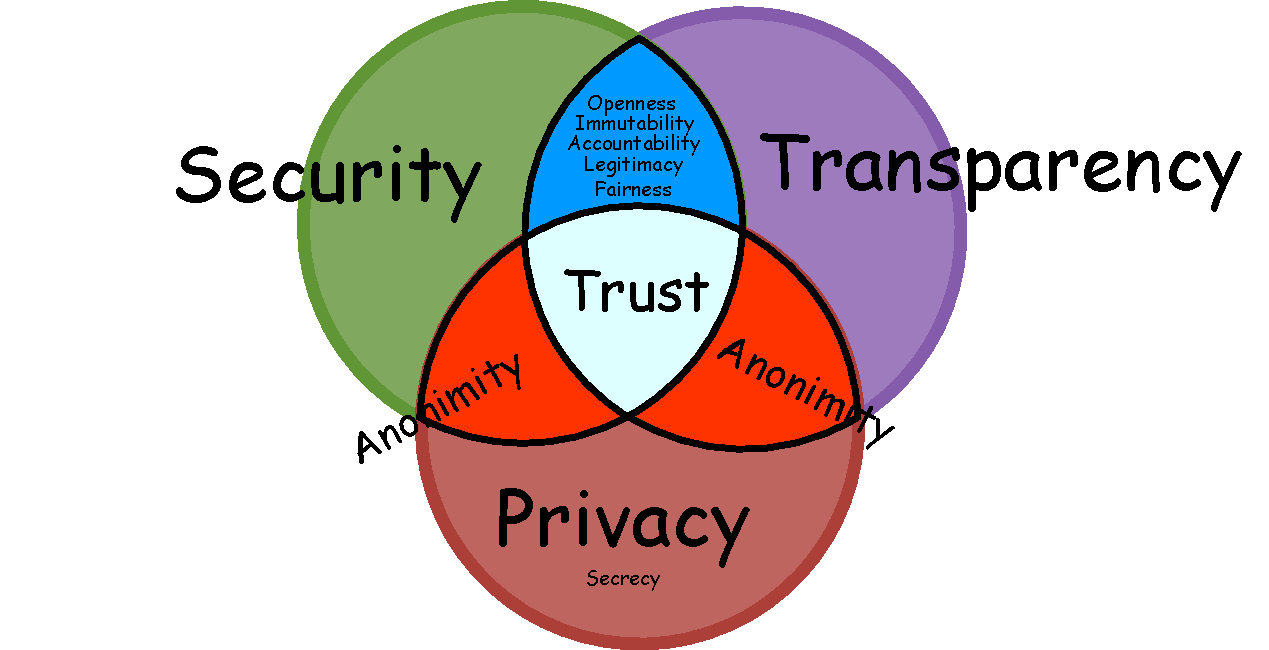
\includegraphics{figures/trust}
\caption{Fundamentals of building trust in election results. Security coresponds to all hardware running services for voting system on behalf of the election officials (guardian). Transparency coresponds to all data which proves conclusevly that ellections results are software independant. Privacy is the quality of decission which is made appart from any observation at the moment (Privacy-Security) and after the vote (Privacy-Transparency).}
\end{figure}
\par
The main difference between a paper ballot and mainstream electronic voting solutions is by a number of machines (including humans) adversary needs to hack to compromise the proofs security-transparency (some policing officials in the paper ballot system) and to compromise the Privacy-Security (an official collaborating with briber). A private company can be isolated from society (NDA agreements, individual selection, etc.), and thus, it makes it easier to hack. On the other hand, hacking software of all election officials who with their social circles cover all society is impossible without being obvious. This leads us to an idea that a secure election system must be open to participation so it could run synchronically on multiple machines at once tied to social circles coercing all society.\par
Most of the voting systems on the literature consider a rather peculiar adversary model. When the voting protocol is modelled as a process, certain parts of the protocol are trusted for verifiability. So voter could get a casting assurance (individual verifiability), and able to validate that only eligible voters had participated, they had voted once, and that the votes had been counted accurately (universal verifiability), but he/she still would need to trust the verifying system as all data for validation can't be published to protect voters privacy.\par
A similar situation is present for ensuring the anonymity of the vote. The anonymity preserving system, for example, a mixnet cascade is often assumed to be held private to avoid malicious activities which can result in the absence of election results. Nevertheless, if we need to trust private mixes, the system although is more disperse it is still centralised. Additional data revealing anonymity can be recorded (as long as authentification is part of a private system) and the organisation can generate necessary proofs of fair elections. Can we avoid those issues in the electronic voting system design?\par
The success of TOR shows that decentralised anonymous network of mixnet cascades can exist allowing to resist government censorship and hiding identity as Edward Snowden from the USA. Other approaches based on mixnets, crowds, onion routing, dc nets are actively developed and deployed. Anonymity of such systems is guaranteed from a realistic point of view of the adversary who would not be able to control every ISP of the world to deanonymize the traffic or control every node providing mix services. Thus with the delocalisation and companionship, we can already today use quite strong means to exchange messages anonymously which we shall reffer as anonymous sockets.\par
However, anonymous sockets yet do not allow to avoid tracking. Unless the electronic voting is an anonymous pool where anyone can vote multiple times, the election voting system is going to have authentification. An attractive solution would be to use linkable ring signature scheme, sign the votes with that and deliver to the vote recorder with an anonymous socket. Unfortunately, linkable ring signatures suffer from their length and computational requirements and thus are not practical. Therefore for a sound system, we shall focus anonymisation of pseudonyms which can be used for authentification of voting messages.\par
Anonymisation of pseudonyms has been studied lately with the context of blockchain and smart vehicle networks VANET. For blockchain CoinShuffle had implemented as additional service which shuffles the transactions making them untraceable. In vehicular networks, the authority would be a benefit to know information on infrastructure quality for further improvement where mix zones for changing pseudonyms is currently actively studied to protect privacy of the car owners. However, the proposed schemes do suffer from the necessity to trust the mixing authority and sometimes also a necessity to trust other participants in the mix. Also, the anonymity of those schemes is of a concern since network anonymisation is often disregarded.\par
In this paper, I will propose a new pseudonym anonymisation protocol using only public-key cryptography which is suitable as substitute for linkable ring signatures. Then I will show how to use them for electronic voting when simultaneously multiple proposals are voted on with PeaceVote system. Furthermore, I will touch on the issue of testing of the system for small communities, distributing software in a trusted manner, as well as how members can be added easily without making the system look complex for the voters and the guardian (maintiner of services). I will also argue that the resulting voting system is strongly software-independent due to the fact the anonymisation of pseudonyms is done in small batches and is strongly anonymous because of openness for participation.\par
\section{Anonimous pseudonyms}
\begin{figure}
\centering
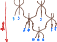
\includegraphics{figures/braiding}
\caption{The pseudonym braiding process. Lines represent pseudonyms, whereas nodes represent braids. The new pseudonyms coming from braids increase their anonymity set size, as shown at the end of the lines with numbers.}
\end{figure}
\par
Imagine an ordinary election. You go to pooling station; greet the gatekeeper who checks your passport; go to a voting booth but then instead of putting your pick for officials you put in the envelope your just generated pseudonym, close the envelope un deliver that to the ballot box. After the ballot officials publish all pseudonyms in bulletin board (roster).\par
The generated pseudonyms in this fashion would have two excellent properties; namely, they would be anonymous and at the same time would be legitimate means to be used for signing votes. We shall call such process braiding as it does have a natural hair-like structure with knots making hairs indistinguishable (in analogy with quantum world it corresponds to superposition of qubits).\par
Braiding, in essence, solves the anonymous authentification issue. However, how can we substitute paper ballot with an electronic one? It may sound like a chicken and egg problem since we need to solve electronic voting problem to do the pseudonym braiding, but it is not quite so. One of the excellent properties of signatures made by pseudonyms is that they are linkable. The linkability allows doing multiple small braids allowing to use multiple small but absolute consensus ballots as shown in the Figure 2. Those small ballots then can be created by multiple different braiding stations which do not need to be trusted allowing them to be trully independent.\par
To avoid a situation where participants pseudonym gets stolen in a braiding process, it is necessary to make individual verifiability as part of the protocol unless other cryptographic proof is provided. That can be achieved if by the end of the ballot it is distributed for every participant to validate and sign thus forming a braid contract. That, however, introduces fragility in the system since any participant can refuse to follow the protocol and thus terminate it while remaining anonymous. This limits the number of participants within the braid.\par
The fragility of the system can be resolved with two instruments. The first one is that the number of participants in braiding shall be kept small. The second one is using a binary search technique to isolate malicious pseudonyms from the honest ones until repeatedly the braiding with different participant sets succeeds. Thus no participant can succeed in paralysing the system, and the protocol can be cascaded to acquire large anonymity set robustly.\par
Nevertheless, who should do the braiding? Multiple systems could fit in as voting protocols based on dc nets and p2p networks with which one could do braiding without any authority. For mixnets, it is necessary to trust the authority that no data is being recorded, which can be used to reveal the anonymity. If only a single mixnet participates which is maintained by the same organization/person, then the anonymity of the vote reduces to the anonymity which would be provided by a conventional mixnet electronic voting system where anonimity is ensured as long as authorithy is honest.\par
The fix for that comes from the fact that we no longer need to trust the mix to do its job since, in the end, participants control with absolute consent whether to accept and sign or discard the braid. That allows forming a system where mixes are distributed over all internet irrelevant of who may use it; To make a braid cascade from multiple mixes and thus resolves any concerns of possible anonymity revealing data as long there is not an initiative to coordinate as that is a threat to anonymity, thus any necessity of that should be eliminated.\par
Openness can be considered as an opposite to coordination. The voting system must be developed from the effort of the community, and as the open-source world had shown monolithic designs fail to attract interest. Thus, on the one hand, it is essential to make the system such that it is easy to start whereas on the other it must not lose the ability to be customized without breaking off from the existing ecosystem. Thus every party would find its place within the ecosystem and so make a pool of available mixers bigger.\par
\section{PeaceVote}
We shall separate the discussion of the proposed voting system in the following categories:\par
\begin{itemize}
\setlength{\itemsep}{0pt}
\setlength{\parskip}{0pt}
\item
Setup;\par
\item
Certification. How to know that one uses the correct software?\par
\item
Registration. How to become a member of the organization?\par
\item
Braiding;\par
\item
Proposing and voting;\par
\item
Counting and verifying;\par
\item
Defence.\par
\end{itemize}
As any voting system, it needs a maintainer, administrator and protector which we shall name as guardian and who is either a single person or an organization itself. The guardian in the PeaceVote system is responsible for the following actions:\par
\begin{itemize}
\setlength{\itemsep}{0pt}
\setlength{\parskip}{0pt}
\item
Starts the services necessary for the voting system;\par
\item
Makes choice on cryptography used (public key system, hashing, encryption, randomness);\par
\item
Makes choice on the method for anonymizing the traffic (TOR or etc.)\par
\item
If applicable, selects mixers for braiding. Sets up a number of participants for the braid;\par
\item
Approves new members for the voting system;\par
\item
Defends the system against DDOS attacks and malicious pseudonyms;\par
\end{itemize}
All those choices must be transparent and available for public scrutiny to impeach the guardian if no confidence had been expressed.\par
Currently, it is considered the best practice to issue SSL certificate on the internet service to make it available for secure access anywhere. That, however, is unsuitable for a voting system where we need to consider such authority to be malicious or even worse selectively malicious. Also, SSL certificates introduce complexity for setting up the system for the guardian, which we would like to make as seamless as possible. This is where the DemeNet project comes in. In place of having a trusted authority, it is better to trust the decentralization of the communication channels.\par
The guardian is interested that the members of the voting system are real so that anyone should be able to verify that the whole community possesses human capacity which can be exercised as power and that unfounded participants do not suppress this power. Currently, governments are actively issuing ID cards with the ability to make digital signatures. Unfortunately, the digital signatures issued by them are only verifiable by a trust service provider adding complexity for the guardian to use them.\par
Ironically the business model of social networks which uses the collected data to individualize us is also making available data on the internet which can be used to assess the reality of the person and provides the means to establish relatively secure communication. Currently, it thus seems sensible to use these relatively secure channels to invite a person to the voting system and at the same time to deliver a trust anchor a \texttt{DemeSpec} file.\par
The \texttt{DemeSpec} file contains only essentials such as the pseudonym of the guardian, cryptographic protocols used, \texttt{UUID} of the self-governing community (deme) which thus is a trust anchor. Since \texttt{DemeSpec} file contains little information, it small and thus it is not a hassle of considering it to be immutable allowing it to be easily distributed. Thus, a potential member could be sure for the genuineness of the invitation from the guardian looking through his trust sources.\par
\begin{figure}
\centering
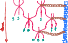
\includegraphics{figures/braidchain}
\caption{Ilustration for formation of immutable ledger BraidChain. For each braid, each participant had validated that his/her new pseudonym is included and that the hash calculated of the local ledger corresponds to the hash specified in the braid. If every participant had agreed on the contents of the Braid (the guardian had collected all signatures), then a braid contract is formed and added to the ledger forming a BraidChain.}
\end{figure}
\par
\subsection{Setting up the voting system}
To set up the voting system, the guardian adds \texttt{DemeNet}, \texttt{PeaceVote} packages and their dependencies to Julia from a trusted repository. The guardian also sets cryptographic primitives for the deme currently provided only by \texttt{PeaceCypher} package.\par
The first step is to create a trust anchor for the guardian, which is contained in the \texttt{DemeSpec} file and saves that:\par
\begin{verbatim}
using DemeNet
using PeaceCypher
demespec = DemeSpec("PeaceDeme",:default,
    :PeaceCypher,:default,:PeaceCypher,:PeaceVote)
save(demespec)
\end{verbatim}
which will create a deme with name \texttt{PeaceDeme}, use \texttt{PeaceCypher} for cryptographic primitives and say that \texttt{PeaceVote} is a peacefounder which for us to simplify discussion currently will not be necessary. (\texttt{PeaceFounder} is a package which deals with defines storage format, notary, cypher, anonymous sockets. It is also package where the interaction between \texttt{PeaceVote} and different services such as \texttt{Recruiters} or a messaging services are defined. It is also environment where experimentation on \texttt{PeaceVote} protocol can take place by function and type piracy.) Additionally by generating a \texttt{DemeSpec} file a private key for the guardian is generated and placed under \texttt{\$HOME/.demenet/keys/uuid/maintainer}\par
The next step is to set up the server. First, a key needs to be generated, which we do as follows:\par
\begin{verbatim}
deme = Deme(demespec)
server = Signer(deme,"server")
\end{verbatim}
where \texttt{Deme} is a primitive which additionally with \texttt{DemeSpec} also had loaded \texttt{Notary} for performing digital signatures and cypher for encryption allowing to establish confidential communications with authenticated Diffie-Hellman key exchange.\par
The next step is to set up the configuration for the braider of the mixnet type. The mixnet braider consists of two parts - a gatekeeper and the mixer. The gatekeeper is responsible for authentification with pseudonyms. It is responsible to redirect connection to the mixer where a new pseudonym is sent and later redelivered back to gatekeeper sorted and forwarded to participants for forming the contract.\par
The guardian needs to specify the pseudonym length and the number of participants for the braid, as well as authentification details for the mixer. Since the mixer is expected to be from a different deme, we define its id with \texttt{DemeID} which contains \texttt{UUID} of the deme togehter with the pseudonym \texttt{ID}, and thus cryptographic primitives can be loaded from the stored \texttt{DemeSpec} file. The configuration then can be created as:\par
\begin{verbatim}
braiderconfig = BraiderConfig(BRAIDER_PORT,MIXER_PORT,
    UInt8(3),UInt8(64),SERVER_ID,MIXER_ID)
\end{verbatim}
where \texttt{BRAIDER\_PORT} and \texttt{MIXER\_PORT} also contain information to establish a socket with server and mixer. \texttt{PeaceVote} only approves integers referring to local ports but with the power of multiple dispatch that can be extended with an external package with its own port type. That is particularly useful in a sense that \texttt{PeaceVote} does not need to specify whether the server is an ordinary server with IP or hidden service in the TOR. The guardian then can specify how ports shall be connected anonymously, whether it is over a TOR network or another way by making, for example, \texttt{BRAIDER\_PORT} an instance of particular type.\par
The next element needed is a configuration of the recorder. The recorder as name states is collecting certified applications, contracted braids, certified proposals and certified votes. The software running it is responsible for preventing redundant information to take part in the ledger. The configuration can be given as follows:\par
\begin{verbatim}
recorderconfig = RecorderConfig([MAINTAINER_ID,SERVER_ID],
    SERVER_ID,REGISTRATOR_PORT,VOTING_PORT,PROPOSAL_PORT)
\end{verbatim}
For this service \texttt{MAINTAINER\_ID}, \texttt{SERVER\_ID} are trusted anchors who are permitted to add new members to the deme. The new members are collected in \texttt{REGISTRATOR\_PORT} who are then able to participate in the braiding. \texttt{PROPOSAL\_PORT} currently is open to all members to submit their proposals (in future it will be configurable for example to board members or etc.). \texttt{VOTING\_PORT} is responsible for recording all certified votes for a particular proposal. Similarly, as \texttt{BRAIDER\_PORT} the \texttt{VOTING\_PORT} contains information on how the anonymous socket can be established.\par
The last part of the protocol is to add a mixer service, which can be used for other demes and on the synchronization port where collected data from the recorder would be published. The full configuration for the PeaceVote thus can be formed:\par
\begin{verbatim}
braidchainconfig = BraidChainConfig(SERVER_ID,MIXER_PORT,
    SYNC_PORT,braiderconfig,recorderconfig)
\end{verbatim}
Currently, only a single braider is provided. It is assumed that the guardian periodically changes the \texttt{BraiderConfig}, thus preventing adversary (even guardian) to collect necessary data from mixers and guardians for revealing the identity of the pseudonym. It is possible to run multiple braiders at the same time, but one then would need to deal with scheduling strategies, etc which are not important for the purpose of this paper for understanding the PeaceVote system.\par
To start the server, the guardian initializes a \texttt{BraidChain} which contains ledger, configuration and deme. \texttt{BraidChain} contains all necessary elements analyses the data collected by the ledger, for example, to count votes and to participate in the \texttt{Deme}.\par
\begin{verbatim}
braidchain = BraidChain(braidchainconfig,deme)
\end{verbatim}
It was a conscious choice that the server and the user use the same configuration data, which shows that the system does not have a hidden state. A new guardian can take the place of the old ones with the data available in the \texttt{BraidChain} and configure further evolution of the community at his/her wish. Though since \texttt{DemeSpec} is immutable, he/she would need to form a new \texttt{UUID} for the deme.\par
Finally, having a \texttt{BraidChain} we can start the server:\par
\begin{verbatim}
system = BraidChainServer(braidchain,server)
\end{verbatim}
which would start all services necessary for the voting system. Since it does not contain any hidden data which one should keep good care of not corrupting (except the server key) it is pure of side effects. That greatly reduces the maintenance costs as in case of problems one can just reinstall the server, put in back the same key (or a new one) and put in the data of the ledger which is stored by every participant everywhere preventing any corruption.\par
\subsection{Certification}
\begin{figure}
\centering
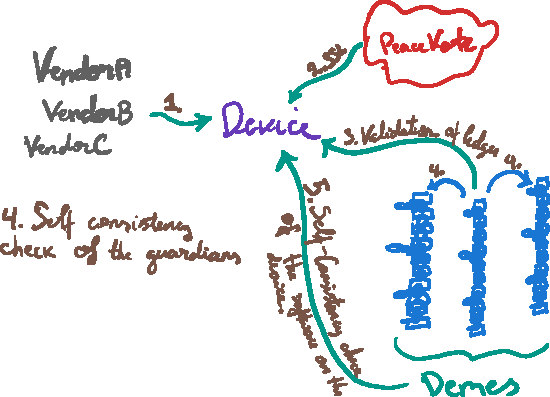
\includegraphics{figures/certification}
\caption{The context of self-certification. Vendor and SSL certificate authority has the freedom to inject any kind of malware/spyware on the device during steps 1. and 2. Nevertheless, the hack would need to be sophisticated because of demes, which store manifest files (containing dependency hashes) of all necessary packages and other trusted guardians. That allows us to do self-consistency check of demes themselves (steps 3. and 4.) and also the software itself on the device as long as software doing the verification is trusted (step 5.).}
\end{figure}
\par
The PeaceVote protocol works because the user uses a trustworthy software on his/her device. Nevertheless, how could users be sure that during the installation of new software, a spyware/malware had not also been added?\par
An ultimate answer to this question for the guardian would be to distribute smartcards which shall be used to ensure that keys are safe and that all signatures made had been logged for accountability of additional device which is necessary to interact with the card.\par
Another way is to trust the software distributor and after the fact test whether the system is self-consistent with the trusted sources selected by the user. For example, a user might receive hashes of the packages certified by demes and could compare that with installed software hashes. That would shrink the area of attack and allow early detection of infected participants since they would certify packages themselves in the braiding process (software hashes could be stored on the \texttt{BraidChain}), which at any time could give evidence that a particular device holds infected code.\par
At the moment, however, such certification of software is not implemented since demes are assumed to be small and incapable of perturbing trustworthiness of certified authorities. It is a reasonable assumption as currently it allows online and mobile banking to function in the practical absence of fraud. Also a simple method by using multiple SSL certificates when installing new software could turn out to be more practical.\par
Another part of the certification is the configuration of the PeaceVote system. If the guardian would be of curios kind, he could make different settings for different participants who would allow revealing the identity of the pseudonyms. Therefore it is crucial that all participants would see the same configuration and could confirm that themselves. We will return to this issue later in the section about braiding and \texttt{BraidChain}.\par
\subsection{Registration}
\begin{figure}
\centering
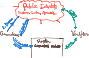
\includegraphics{figures/registration}
\caption{The registration and external verification process with public roster. First, registration with recruitment token is shown, which produces an entry in the roster where the guardian certificate of the pseudonym and data containing information to contact the person. The verifier can use the roster to check the realness of a member and inquire the member that he/she indeed owns the specified pseudonym.}
\end{figure}
\par
To take part in the deme the guardian or it's delegated authority needs to sign users pseudonym. From the guardian perspective, she/he is troubled with distinguishing genuine application over bots. In an ideal world, the pseudonym before sent to the guardian would be signed by a personal smartcard or by a state authority confirming users identity. However, the ideal world is not always available, and if smartcards are available, those require developer power and some cheesy subscription model which together kills accessibility.\par
A solution to such problem could be by using our online presence in different social networks, let it be Facebook, Twitter, Google, LinkedIn, OpenID, etc. which generally do provide enough information for a person to assess whether the person is real or a bot. However, it is close to impossible to make a computer program which would do that automatically.\par
The guardian does have three options. The first one is upon application the guardian checks the identity online and tries to establish online communication over one of the communication channels to check whether the person applying is not a bot which had borrowed a random identity and on such assessment would issue a certificate. The second option is that the guardian upon a request delivers a token to the phone, email, etc. which can be used to register to deme. The last option is to allow everyone in and then kick off those who are not real.\par
The first option is tedious but might be necessary in case one needs high assurance of the identity (investor board meeting). The last option of kicking off unreal members are possible by the guardian issuing order that all pseudonym braiding should restart from their anchors. The second option of delivering a token upon a request is most practical one which is what in one form or another we use daily, and this is the one we shall rely on the daily basis for \texttt{DemeNet}.\par
The registration for the \texttt{DemeNet} with tokens is currently implemented with \texttt{Recruiters} package. The algorithm of it is as follows:\par
\begin{itemize}
\setlength{\itemsep}{0pt}
\setlength{\parskip}{0pt}
\item
The guardian starts the server certifier service and the token receiver service.\par
\item
A potential member is sending the application to the guardian or his delegated trusted people.\par
\item
After a review which could also be automatic if the phone number is provided or other trusted source of communication, the applicant receives a token, \texttt{DemeSpec}, and the information to connect to the registration server. The token is sent to the certifier service confidentially.\par
\item
The applicant generates a key, establishes a secure connection to the guardian certified certifying service and sends his pseudonym and token.\par
\item
If a token is found, a certificate is created by the server key and the pseudonym is added to the roster. Additionally, a log file is kept on the communication channels and information, which had been used as a basis to issue the registration certificate.\par
\end{itemize}
It is important to note that to use \texttt{Recruiters}; the guardian is responsible for doing the piping of issued certificates of the server to roster stored on the \texttt{BraidChain}. As this and other steps for configuration are so common, it is recommended to use \texttt{PeaceFounder} package which integrates \texttt{PeaceVote} with \texttt{Recruiters}.\par
A great thing with tokens is that one can send an invitation to people without them making to do work and if they decide to apply, they can do that instantly. This is particularly great to form the demes spontaneously just by starting a server, sending invites to the email, braid and vote. Users would still need to install an app, but as it would be useful for multiple demes in the long term such inconviniance would be treated as the cost of installing a web browser, email client, etc.\par
\subsection{Braiding}
\begin{figure}
\centering
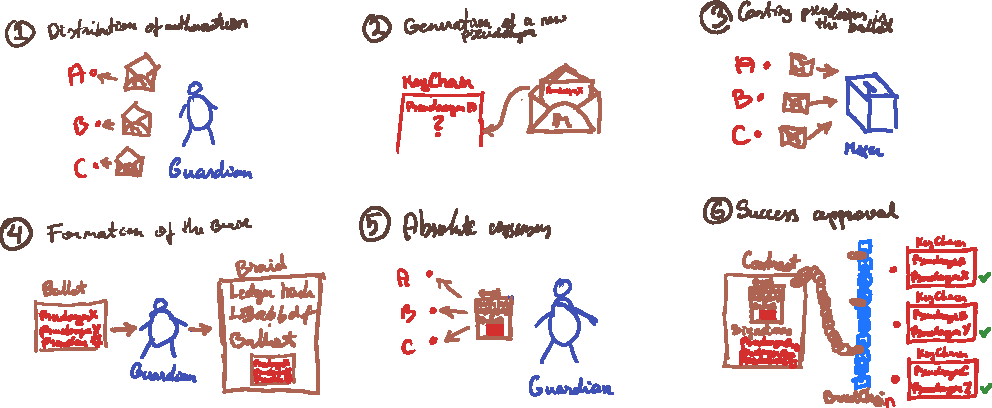
\includegraphics{figures/braiding2}
\caption{Ilustration of the braiding protocol. 1. The guardian arranges seeking participants into single potential braid and redirects socket to mixer. 2. Each participant generates a new potential pseudonym and 3. delivers that to the mixer. 4. Then mixer delivers randomized ballot of pseudonyms to the guardian who froms a Braid additionally adding current BraidChain hash. 5. The same braid is delivered to every participant to validate and to sign. 6. If succesful guardian collects all participant signatures, forms a Contract and puts that in the BraidChain. Then each participant synchronizes the BraidChain and either saves or discards the new pseudonym.}
\end{figure}
\par
At his point the members have been registered, they have loaded the \texttt{DemeSpec} file sent to them together with an invitation. They have synchronized their ledger with the guardian (one way) with the provided information in the invitation, for example, a port and IP address. The ledger contains \texttt{BraidChainConfig} certified by the guardian.\par
The user loads the configuration file, and its first step is to gain anonymity by creating a new pseudonym during braiding. All keys for the pseudonyms are stored locally, which as we will see is essential for dynamism in the voting system - braiding shall not limit voting and voting braiding. The storage unit is called \texttt{KeyChain} and can be initialised as follows:\par
\begin{verbatim}
keychain = KeyChain(deme)
\end{verbatim}
which will load keys from \texttt{\$HOME/.demenet/keys/uuid/*} and sort them in their chronological order.\par
When the keys are loaded with the braidchain the user can gain anonymity by braiding which can be simply done as:\par
\begin{verbatim}
braid!(braidchain,keychain)
\end{verbatim}
This simple command in the context of \texttt{SynchronicBallot} is performing a following algorithm:\par
\begin{itemize}
\setlength{\itemsep}{0pt}
\setlength{\parskip}{0pt}
\item
The user authentificates with the gatekeeper in both directions with the current pseudonym and encrypts the connection.\par
\item
The gatekeeper forwards the connection to the mixer with which it has authetificated and encrypted.\par
\item
The user using the same socket is now authenticating the mixer and establishing an encrypted connection.\par
\item
The user generates a new key and sends the pseudonym to the mixer\par
\item
The mixer collects all pseudonyms from the participants, sorts them and sends them back to the gatekeeper.\par
\item
The gatekeeper forms a braid from all collected pseudonyms. Additionally, the guardian adds a hash of the current ledger. (Other relevant metadata can also be added such as time up to which the braid must be published to the ledger, etc.)\par
\item
The participants validate the braid verifying whether their pseudonym is within the braid and also verifying that the hash of the local ledger is the same as hash put in the braid. If validation succeeds the participant signs the braid and delivers the signature to the gatekeeper.\par
\item
If braiding went successful, the gatekeeper collects all signatures verifies them and publishes the \texttt{Braid} contract to the \texttt{BraidChain}. If unsuccessful, the procedure is repeated with variations of a set of participants, perhaps of the mixer, etc.\par
\end{itemize}
In this procedure, the user can be the guardian certified pseudonym or any anonymous pseudonym which follows this procedure. When the procedure is repeated, it becomes crucial to anonymize the IP address of the connection as that link to the previous pseudonym. It can not be up to users deciding how they anonymize a socket because anonymity loves company and thus the guardian specifies the serveice, for example, TOR, with in the \texttt{BraidChain}\par
Additionally, during the braiding participants do certify the ledger of the \texttt{BraidChain}. This makes the information stored on the ledger immutable to any adversary and ensures that all members see the same ledger. \texttt{BraidChain} thus is convenient as a place where the guardian could distribute the configuration of the voting system, prohibiting deanonymization attacks by a vicious guardian. Additionally, a \texttt{BraidChain} is an excellent place to store other information necessary for certification such as trusted software hashes or other \texttt{DemeSpec} files and thus forming a real deme network or simply \texttt{DemeNet}.\par
\subsection{Proposing and Voting}
\begin{figure}
\centering
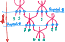
\includegraphics{figures/voting}
\caption{Proposing and voting in the BraidChain. First, an eligible participant creates and puts a proposal to be included in the BraidChain. The position in the chain sets current (newest) pseudonyms as a legitimate set of participants shown as an intersection with blue nodes. Those pseudonyms at any time at the future (unless the proposal has a deadline) voters can use to issue their certified votes and deliver them anonymously to the vote recorder.}
\end{figure}
\par
After braiding each member owns a chain of anonymized pseudonyms \texttt{KeyChain} which can be used to sign messages in our situation votes. However, each pseudonym is itself anonymous and part of the \texttt{BraidChain} which one should one use? Is the newest one enough?\par
Before the vote, an eligible member makes a \texttt{Proposal} with approved pseudonym of the deme (by default all \texttt{PeaceVote} members can make a \texttt{Proposal} with their pseudonym anchor). The \texttt{Proposal} for the \texttt{PeaceVote} is one of the most abstract it can be for a voting system. In itself, it contains two important properties - how the votes for it are going to be counted and what is the input from the user. \texttt{Proposal} could be a single question with multiple options, or it is a whole survey a list of questions for which voter is forced to decide on the priorities of the organisation in an interconnected way having a constraint like in quadratic voting.\par
The \texttt{Proposal} again is registered to a \texttt{BraidChain} for tamper resistance to avoid a situation where a proposal gets changed to deliver an opposite outcome. Additionally, it defines a set of pseudonyms by the position in the \texttt{BraidChain} by making interesection with current (newest) pseudonyms. This way, each participant would have only one vote.\par
The voter does the last step. He/She synchronises his/her \texttt{BraidChain} with the guardian and checks its integrity (see next subsection on validation). Then he filters out the proposals from the BraidChain which are then parsed by user application of the PeaceVote and shown on the screen. To vote user selects a \texttt{Proposal} and fills the form expressing the choice producing the option:\par
\begin{verbatim}
option = Vote(index,choice)
\end{verbatim}
where \texttt{choice} is the result of filling out the specific \texttt{Proposal} and is assigned to proposal with \texttt{index} in the \texttt{BraidChain}.\par
The vote is created by digitally signing the option with corresponding pseudonym as specified by the index in the option:\par
\begin{verbatim}
vote = Certificate(option,keychain)
\end{verbatim}
Finally, voter delivers the vote anonymously:\par
\begin{verbatim}
record(braidchain,vote)
\end{verbatim}
where TOR or similar service is used behind the scenes as specified by the guardian in the \texttt{BraidChain}.\par
\subsection{Validating and Counting}
When the voting period ends, it is time to collect votes, validate their eligibility and count them. The votes themselves can be either published in the \texttt{BraidChain} immediately, can be delayed and published later or can be kept in secret which can be useful for implementing anti-bribery and anti-coercion mechanisms (see the next subsection). The second part when all votes had been collected is to validate them, which means that the vote had been signed by a current pseudonym specified by the place of the \texttt{Proposal} in the \texttt{BraidChain}. The last part is to count them as defined by the type of the \texttt{Proposal}.\par
Assuming that all votes had been collected (which by default in \texttt{PeaceVote} are stored on the BraidChain providing tamper resistance) the next step is to validate the \texttt{BraidChain} which can be separated in following steps after the ledger had been properly synchronised:\par
\begin{itemize}
\setlength{\itemsep}{0pt}
\setlength{\parskip}{0pt}
\item
Parsing. At this step ledger which is just an array of byte vectors \texttt{Vector\{Vector\{UInt8\}\}} is parsed to a \texttt{Vector\{Union\{Certificate,Contract\}\}} where certificate/contracts contain the document and its signature(s):\par
\end{itemize}
\begin{verbatim}
parsedledger = parse(braidchain.ledger)
\end{verbatim}
\begin{itemize}
\setlength{\itemsep}{0pt}
\setlength{\parskip}{0pt}
\item
Validation of immutability. Move through each element in \texttt{parsedledger} and validate that hash specified in the \texttt{Braid} agrees with hash of the local ledger and return integer \texttt{m} up to which that is true:\par
\end{itemize}
\begin{verbatim}
m = followhashes(parsedledger,deme.notary.hash)
\end{verbatim}
\begin{itemize}
\setlength{\itemsep}{0pt}
\setlength{\parskip}{0pt}
\item
Attestation. At this stage, the certificates and contracts are cryptographically verified producing \texttt{Vector\{Union\{Intent,Consensus\}\}}. \texttt{Intent} and \texttt{Consensus} contain the documents and IDs of who issued the signatures. The operation for this procedure can be performed as follows:\par
\end{itemize}
\begin{verbatim}
verifiedledger = attest(parsedledger,deme.notary)
\end{verbatim}
\begin{itemize}
\setlength{\itemsep}{0pt}
\setlength{\parskip}{0pt}
\item
The last step is to validate the ledger for its integrity. The result of validation is an index until which the ledger is considered valid. The validation procedure can be described as follows:\par
\begin{itemize}
\setlength{\itemsep}{0pt}
\setlength{\parskip}{0pt}
\item
Initialisation. Create an empty set for current pseudonyms, mutable set of parameters - current authorities who can issue member certificates, a current hash of the ledger and iterate through each element in a verified ledger.\par
\item
If the element is \texttt{Intent\{Config\}}. Validate that it comes from the guardian and if so, update the mutable set of parameters with approved authorities who can issue a new member certificate. Else break.\par
\item
If the element is \texttt{Intent\{ID\}} and is signed by current authorities, add the pseudonym to the current pseudonyms. Else break.\par
\item
If the element is \texttt{Consensus\{Braid\}} and is signed by N current pseudonyms where N is a number of new pseudonyms, then swap pseudonyms form the current pseudonym set as specified by the braid. Else break.\par
\end{itemize}
\end{itemize}
\begin{verbatim}
n = followbraids(verifiedledger,deme.demespec.guardian)
\end{verbatim}
In case the \texttt{n} or \texttt{m} is smaller than the length of the ledger end of the ledger is being cut, the ledger again is synchronized with the guardian certified server and the procedure repeated for the end of the ledger.\par
After the validation of the ledger, we can operate on the data. First, we can extract the proposals from the verified ledger which one does as follows:\par
\begin{verbatim}
pindexes = getproposals(verifiedledger)
\end{verbatim}
which will return the indices of the proposals in the ledger. For each proposal index, first, we can get the corresponding \texttt{Proposal}:\par
\begin{verbatim}
proposal = verifiedledger[pid].document
\end{verbatim}
The votes can be obtained by:\par
\begin{verbatim}
votes = getvotes(pid,verifiedledger)
\end{verbatim}
where votes corresponding to the \texttt{Proposal} with index \texttt{pid} are filtered out of the \texttt{BraidChain}. The proposal may contain time when the voting period ends which can be incorporated by slicing the \texttt{verifiedledger}.\par
The final procedure is counting. To do so, the user does:\par
\begin{verbatim}
tally = count(proposal,votes)
\end{verbatim}
where one can implement whatever method of counting one wishes. Whether votes can be changed after cast, whether it is a preferential ballot, or multiple question ballot with a constraint, for example, a budget, quadratic voting. All these are trivial to implement for the message based voting system.\par
\section{Adversaries and defence}
I identify three types of attacks adversary could exercise. The first one is an attack on the network infrastructure. In this category, we have DDOS attacks and attacks on the TOR network to reveal the real identity. The second type is infiltrator attack where the adversary is part of the system in this case, either guardian, mixer, or some coalition of members. The third kind is an attack on the secrecy of the voter. First, it could be malware/spyware on the device, or it could be coercer/briber who convinces the voter to collaborate.\par
\subsection{Attacks on network infrastructure}
Online systems are prone to attacks which can make them offline. Often that is achieved by buying botnet to make requests on the services until they do overload, which is the definition of a DDOS attack. No online system is protected from this kind of attack. Nonetheless, one can always reason about the costs.\par
The characteristics of PeaceVote system allows distributing the load over an extended period of time. The braiding procedure which requires a stable network and stable operations of gatekeeper and mixer are not required to happen on the election day. Thus DDOS attacks on braider become increasingly costly.\par
The other DDOS attack on election day can happen on the vote recorder. In the current design of PeaceVote, the remedy is to use shields which filter out valid votes from fake ones. Since all authentification data is in the BraidChain which is available to everyone, such shields would be easy to set up if necessary.\par
Another kind of attack we need to be aware of is the attack on the network anonymizer, for example, TOR network. It is known that if ISP is all-powerful and records all inputs and outputs the identity can be deanonymized in some given time period. Alternatively, there could be infiltrator attacks on the TOR network itself, which could make connections with inputs and outputs. The question is how plausible it is?\par
We can consider Edward Snowden's location as a target of the USA government. The information on his IP address could quickly lead where he is located; thus, he may just refuse to use it. On the other hand, he knows that TOR network makes his IP address untraceable allowing him to use internet and to participate in discussions on the media, conferences and etc. where ends of TOR are assigned to his identity. To this point, Edward Snowden had not yet been found proving the strength of anonymity of the TOR network.\par
\subsection{Infiltrator attacks}
The other kind of attacks is when adversary had acquired control over some part of the infrastructure, including members. Realistically that could happen due to some security flaw which allows gaining control of the servers or the people themselves. In any case, it is necessary that the adversary can be detected, isolated and its attack defended. We shall consider three kinds of adversaries and their coluborations. A vicious guardian, mixer and coalition of a subset of members.\par
The isolated guardian as the adversary can block the accessibility of services and filter out which votes he would like to accept with the recorder and also accept fake identities. In the case when the guardian blocks accessibility it could turn out to be tricky to detect whether it is due to him being corrupt or due to receiving a DDOS attack. For the later a shield(s) can be used to deffend a DDOS attack by a wise guardian. Thus its impeachment due to DDOS attack should not be sympathized with.\par
The guardian is also responsible for the acceptance of new members. A legit question for a participant would be whether those are actually real. This question can be tested statistically. To do so, a random set of participants are selected, and those identities then are matched with the guardian published contact details which should lead to some social network or etc. The last step is then to contact those people to see whether they know that they are part of the deme.\par
The other malicious action which guardian could do is to accept for recording only those votes which are of his liking. To detect such situation the vote can be delivered first to a policing authority with TOR which then tries to publish it to the recorder. If it fails, it sends the vote to the next policing authority which again tries to publish that. In this way, a consensus of corrupt guardian would be created and thus he/she could be impeached.\par
The guardian is also responsible for ensuring that mixer and members are not breaking down the service. In the case of the mixer, the most malicious thing would be to alter the ballots by inserting his own pseudonym or just slightly corrupting it. In such action, the braid would come to participants where one would find it corrupt and thus refuse to sign breaking the protocol. At this point, the guardian does have a hard time deciding on whom to blame.\par
At this point, the guardian has two things he can try. First one he can try to repeat the braiding procedure by excluding those who refused to sign the ballot until the braiding protocol succeeds. And later one letting those who terminate the protocol braid with themselves. If that fails a significant number of participants had entered the braiding prison, the guardian might suspect that the mixer is corrupt, which he can let to be publically known (for example, stored in the \texttt{BraidChain}). The solution here is just to issue a new configuration which uses a new mixer which a trustworthy guardian should do regularly anyway, which we will now consider.\par
The next type of adversary is one who controls the mixer and the gatekeeper. Such a situation quickly rises when in the PeaceVote protocol mixer is self-hosted by the same guardian. In such a situation, adversary can silently record additional data which allows revealing identities with corresponding pseudonyms. To prevent the rise of such a situation, the participants may ask that the mixer is changed regularly, which is served by trustworthy or unaccessible guardians on the internet.\par
\subsection{Secrecy attacks}
The last type of adversary is one who attacks the secrecy of the voter. In paper ballot system only the voter knows the secret on how he voted on and thus the briber/coercer is powerless on whether the voter is telling the truth unless he uses a lie detector or something. In electronic voting, there is no way to ensure that the voter is voting on the device without adversary behind his back observing. Additionally, the adversary could be operating anonymously behind the internet or the device the voter uses could have malware/spyware.\par
To avoid malware/spyware, a certification procedure is used. The goal is to avoid malware/spyware to come to form the PeaceVote protocol, which is open to extension with different cryptographic methods, network anonymizers and etc. As described in the certification section, the PeaceVote protocol could perform self-consistency checks with already trusted sources before using a new component. Initial trust source as a package repository would be provided by the distributor of PeaceVote.\par
The next type of malware/spyware could come from the device itself. First, it could come from another application on the device. To avoid such situations, vendors are already putting applications in containers which do have restricted access. Thus it is vendors responsibility that device does not have a malware on it. That currently, for example, allows mobile banking to happen without significant issues of fraud. Thus why not make the same trustworthiness assumption on electronic voting?\par
The first most dangerous attack on secrecy is by anonymous briber/coercer. The briber can exchange a certain amount of money for an exchange of vote. Additionally, for the PeaceVote protocol, the briber could ask for the pseudonym key itself which they could use for unlimited voting while still having backing from a real identity.\par
To fight the selling of pseudonyms online, we need to prevent its extraction from the device. It could be made possible that the keys are stored and generated during braiding in the smartcard itself, thus preventing its users from selling their pseudonyms. The identity pseudonym then could be signed by a vendor issued key on the card to prove that issued key and derived ones in the process of braiding are not possible to be extracted. The card itself then can be verified with biometrics (with which I mean one signs video chat with the key on the card, etc.) that it does belong to a real person.\par
Not able to buy pseudonyms the briber/coercer would turn to buy votes instead. In the case of anonymous adversary, the strategy would be that the vote would be collected by it before delivered to the recorder in that way, ensuring that an existing vote is not smuggled into him. Additionally, he may only give payment after the elections had ended and the bought vote had been accurately voted on.\par
To solve such issue, most voting systems implement some form of receipt freeness or as I like to simplify prooflessness. In the PeaceVote system prooflessness can be implemented if the votes are not published but only the tally at the end of the vote. Then one can implement the ability to silently change the vote after it had already been sold to briber/coercer. But in doing so, one sacrifices transparency, particularly, universal verifiability of the voters for prooflessness. The votes though themselves can be universally verified by the permitted personnel.\par
Perhaps a succeful compromise could be achieved if the voter would have a choice whether the vote is going to be public or hidden. By default, the voter would publish the vote for everyone to see, but in the case, there is an opportunity to sell it to the briber he/she does so. After the fact he/she submits a new vote which remains hidden from everyone except the guardian (or his/her approved authorithy) who after elections issues correction to the public result as a tally.\par
As long as the election result, who happens to be elected and who not, is determined from the publically available ones there would be no point to question the integrity of the guardian who counts the hidden votes. Furthermore, to prevent maliciousness of the guardian, an independent auditor could be used to recount the correction.\par
Similarly, the same bribery/coercion mechanism could work in person as long as the briber is not looking behind the back of the voter and then collect the device until the end of elections. To prevent such scenario, the voters should have the ability to defend themselves, for example, by issuing a tagged vote (the briber/coercer would not know if the used pin code to a smartcard triggers tagging) in the presence of briber/coercer which would give a signal to authorities that a possible crime is happening allowing to punish the criminal.\par
\section{Comparissions with different frameworks}
\subsection{A letter to a loosing candidate}
Dear Mr X\par
The elections had ended, and your candidacy had not gained significant support from the people. In this letter, we shall explain why we believe that the elections had happened honestly.\par
First of all, only eligible citizens were able to make a valid vote. The participants were independently verified with a public rooster, ensuring that each citizen had only one vote and no information was received of a person not able to hold necessary credentials. Smart cards were used to prevent the selling of the voting credentials by just copying the keys.\par
The privacy of the voters was ensured with the process we call the pseudonym braiding. What it does is it creates multiple unrelated knots which even we as election authority are unable to untie unless we had collaborated with all independent mixers producing the anonymity. In this process, no voter could lose their credentials due to the last step of the protocol being collecting absolute consent of validness from the participants to form a braid. This process additionally ensures that the voting ledger is immutable and every voter sees the same information on how to vote.\par
Each voter by signing their option with pseudonym delivered vote with TOR to the vote recorder ensuring their anonymity. After the election, it was published to everyone accessible ledger, where the voter by typing in his pseudonym on another device could ensure that the vote had been recorded accurately. Additionally, voters had the ability to deliver the votes to their pseudonym preassigned secret vote recorder to prevent vote-buying and coercion where they also obtained cryptographic assurance that their vote had been cast as specified on the device. The braiding process during the elections ensured that no vote was deleted by anyone, even us.\par
After the elections, we present you with a list of public votes stored in a braidchain in which you can validate that results had not been tampered with, that every vote is legitimate, and do the count of them to produce a public tally. The votes collected by secret vote recorders were counted by multiple independent verifiers producing a correction tally to the public one.\par
In the end, looking of the complete tally, we conclude that your candidacy had lost with a margin larger than a possible error in the process to ask for a recount of secretly collected votes.\par
We are sincerely sorry for your loss,
Election committee representative Y\par
\subsection{A framework for comparing different voting schemes [15]}
This framework evaluates the voting systems in three categories. Confidentiality which characterizes the privacy of individual voter and as well the aggregate to protect from coercers and bribers. This approximately corresponds to Privacy circle in Figure 1. Integrity which discusses the evidence provided during and after the elections. This part fits in Security-Transparency intersection. And last availability which fits in Security circle previously discussed. Each of these criteria voter describes with regards to the power of authority which is a welcome addition for considering the trustworthiness of voting systems.\par
\begin{itemize}
\setlength{\itemsep}{0pt}
\setlength{\parskip}{0pt}
\item
[P1] \textit{Malware on voting device is unable to violate ballot secrecy.} Never holds. The malware is capable of seeing the pseudonyms used for voting and further on deliver them to an adversary.\par
\end{itemize}
I oppose this issue on the grounds that for malware mobile banking is immediately more profitable than profit gained by selling voters privacy.\par
\begin{itemize}
\setlength{\itemsep}{0pt}
\setlength{\parskip}{0pt}
\item
[P2] \textit{Malware on voting device is unable to manipulate votes.} Holds. The information is typed in on the device for forming the vote. Thus malware can change the vote what is sent to \texttt{BraidChain}. But the voter is capable knowing his pseudonym to see what vote is stored on the \texttt{BraidChain} knowing his anonymous pseudonym for the proposal and if necessary re-vote.\par
\end{itemize}
But if additional secret ballot box is used this property no longer holds as malware can deliver the new vote there. In this case, smartcard which stores the log file accessible to authorized officials could remedy this problem.\par
\begin{itemize}
\item
[P3] \textit{Voter is able to keep their ballot as secret.} Holds even when all authorities are misbehaving because mixes are public. To reveal anonymity of the pseudonym and thus votes, the guardian and all braiders must collaborate in advance by recording additional data. The braiders are not part of the authority since those are public and verifiable.\par
\item
[P4] \textit{Voter is unable to prove to a large-scale vote-buyer how they voted.} Holds when none of the authorities is corrupted, if additional secret ballot box is used. The large-scale vote buyer can use the information available publicly seeing how each pseudonym had voted and that his vote had been counted accurately. To deal with that, an additional secret ballot is proposed where voters can re-vote without revealing the pseudonym. It's existence, but not use, would prevent briber from being sure that his vote had not been discounted.\par
\end{itemize}
Additional security can be gained if multiple secret ballots are used and those are assigned to individual pseudonyms at random (for example by the first letter in the pseudonym). In that way, the large scale vote buyer to work effectively would need to infiltrate the majority of those authorities. Otherwise, they would need to make a condition that only pseudonyms which use a particular secret ballot would be accepted for vote-buying. That would raise eyebrows to that specific authority.\par
Moreover, to prevent selling the pseudonym and to prevent the voter from proving that he/she does own it, a smartcard can be used for storage, braiding and voting.\par
\begin{itemize}
\item
[P5] \textit{Voter is unable to prove to a large-scale vote-buyer that they wasted their right to vote.} Holds when none of the authorities is corrupted, if additional secret ballot box is used. The voter can directly send their vote to a secret ballot box, without revealing to the briber that they voted. Reasoning similar to P4.\par
\item
[P6] \textit{Voter is unable to prove to their spouse how they voted.} Holds when none of the authorities is corrupted, if additional secret ballot box is used. The voter can re-vote with secret ballot box after as long as the spouse gives a window for secrecy with the voting device or smartcard used. Reasoning similar to P4.\par
\item
[P7] \textit{Voter is unable to prove to their spouse that they wasted their right to vote.} Holds when none of the authorities is corrupted, if additional secret ballot box is used. The voter can directly send their vote to a secret ballot box, without revealing to the spouse that they voted as long as the spouse does give a window for secrecy with the voting device or smartcard used. Reasoning similar to P4.\par
\item
[P8] \textit{Voter can ensure their ballot is not accidentally spoiled.} Holds, even if all authorities are corrupted. Each voter sees public ledger where he/she can see their vote to be recorded accurately.\par
\item
[P9] \textit{Voter can ensure their vote is recorded as cast.} Holds, even if all authorities are corrupted. Each voter sees public ledger where he/she can see their vote to be recorded accurately.\par
\item
[P10] \textit{Voter can detect if their vote is displaced (deleted, replaced or pre-empted).} Holds, even if all authorities are corrupted. The ledger is immutable due to it's hash added to every single braid. Thus votes recorded could no longer be removed.\par
\end{itemize}
In the case of the secret ballot, a hash of the vote and it's the corresponding value of the vote is published. That allows an individual voter to verify the cast. The hashes are recorded to the braidchain to ensure immutability.\par
\begin{itemize}
\item
[P11] \textit{The tally is counted correctly from recorded votes.} Holds, even if all authorities are corrupted. Each voter can download the full ledger and do the count themselves.\par
\item
[P12] \textit{No ballot stuffing.} Holds, even if all authorities are corrupted. Each vote is signed by anonymous pseudonym whose legitimacy is guaranteed by absolute consensus in the braiding protocol. Thus pseudonyms not approved by authority does not enter in the system. The authority also publishes the pseudonym anchor with identity in a roster. That way, anyone can verify that approved members of the system are legitimate.
In case additional secret ballot box is used, independent verifiers are essential to ensure that authority is not misbehaving computing the tally. The published hashes on the braidchain ensure that every vote can be accounted for.\par
\item
[P13] \textit{Denial-of-service resistance.} Holds, even if all authorities are corrupted. The braiding of pseudonyms happen over a longer time period than the voting, thus DDOS attack on services must be persistent over this extended period making them impractical. The recorder of the votes can be shielded with a relay like service as all legitimate pseudonyms able to publish votes are available publically.\par
\end{itemize}
\section{Discussion}
Electronic voting is a very complex problem which can have great consequences on democracy. Each system comes with its own need of expert knowledge, and thus discussion of the most trustworthy design publically could potentially be steered to insecure systems to the benefit of capital. It is thus vital to battle test voting systems and start small. As the power of democracy built with them becomes more significant, they stand a chance to gain interest in hacking by corporations and capital who could be interested that there would not be such thing as a society.\par
The PeaceVote voting system, while complex is the first system which achieves true transparency, security and privacy. The trust on it is derived from those components and not from trusted personnel. The system is strongly software-independent for voting. The system does not contain a hidden state and can be reset/restarted at any time with the publically available data. The guardians are powerless. Their wise actions and reputation are what matters for a new guardian to show up and impeach the old one. The design allows us to have a giant mixnet cascade, which is possible due to openness and introduced a process called braiding. The system scales in two directions. Though one may wish to fragment it to some regions, etc. to limit the processing power and storage needed for participants.\par
Although complex it is one of the easiest to set up. In contrast to blockchain ideology, it is fine to start small. The trust is built from wise actions and not from competitions of wasted work (PoW) or legitimatized inequality (PoS). A new guardian can start with a single raspberry pi and use automatic configuration which would generate a key for the deme and for the server, which does not require a permanent IP address or SSL certificate to be trustworthy. Then to use it, voters only need to install an application on their smartphones which would allow participating in different demes.\par
The PeaceVote voting system also allows easy to be used for whistleblowing where in place of issuing votes, one can just sign a leaked document with a pseudonym. This could be particularly useful for corporations which, according to most common European laws require that whistleblowing should be possible and even encouraged to prevent ill effects on society. Ensuring strong anonymity of whistleblowers is what PeaceVote can do.\par
The infrastructure around PeaceVote is more generic than the voting itself. Particularly DemeNet addresses the issue of requiring SSL certificate issued by an authority which is substituted with self-consistency and directly distributing the ids of the guardians. That allows easily to add other services like chatting, messaging service, a localised search engine. A news distributor where the voting could allow for subscribers to decide upon what content they would like to see and thus giving the initiative to pay subscriptions.\par
To conclude, the internet had become a dystopia, full of tracking and suspicion of sincerity of information. It is time to come together and start to found some peace with the world around us. It is time organise for the trust and breaking systematic media suppression of public opinion suppression from the state. It is time to organise to self organise. Could \texttt{PeaceVote} fill that hole?\par

\begin{thebibliography}{9}
  
\bibitem{Adida2016} Ben Adida. 2006. Advances in cryptographic voting systems. Ph.D. Dissertation. Massachusetts Institute of Technology, USA. Advisor(s) Ronald L. Rivest.
\bibitem{Anderson1995} Anderson R., Needham R. (1995) Programming Satan's computer. In: van Leeuwen J. (eds) Computer Science Today. Lecture Notes in Computer Science, vol 1000. Springer, Berlin, Heidelberg
\bibitem{Chaum1981} Chaum, D. L. (1981). Untraceable electronic mail, return addresses, and digital pseudonyms. Communications of the ACM, 24(2), 84-90.
\bibitem{CoinShuffle2014} Ruffing, T., Moreno-Sanchez, P., \& Kate, A. (2014, September). Coinshuffle: Practical decentralized coin mixing for bitcoin. In European Symposium on Research in Computer Security (pp. 345-364). Springer, Cham.
\bibitem{Danezis2003} Serjantov, Andrei \& Danezis, George. (2003). Towards an Information Theoretic Metric for Anonymity. 2482. 10.1007/3-540-36467-6\_4.
\bibitem{Danezis2008} Danezis, G., \& Diaz, C. (2008). A survey of anonymous communication channels (Vol. 27, p. 30). Technical Report MSR-TR-2008-35, Microsoft Research.
\bibitem{DolevYao1983} Dolev, D., \& Yao, A. (1983). On the security of public key protocols. IEEE Transactions on information theory, 29(2), 198-208.
\bibitem{Franck2008} Christian Franck (2008). New Directions for Dining Cryptographers. MSc thesis.
\bibitem{GolleJuels2004} Golle, P., \& Juels, A. (2004, May). Dining cryptographers revisited. In International Conference on the Theory and Applications of Cryptographic Techniques (pp. 456-473). Springer, Berlin, Heidelberg.
\bibitem{Gritzalis2002} Dimitris Gritzalis (2002) Secure Electronic Voting
\bibitem{PublicEvidence2017} Bernhard M. et al. (2017) Public Evidence from Secret Ballots. In: Krimmer R., Volkamer M., Braun Binder N., Kersting N., Pereira O., Schürmann C. (eds) Electronic Voting. E-Vote-ID 2017. Lecture Notes in Computer Science, vol 10615. Springer, Cham 
\bibitem{Rivest2008} Rivest, R. L. (2008). On the notion of ‘software independence’in voting systems. Philosophical Transactions of the Royal Society A: Mathematical, Physical and Engineering Sciences, 366(1881), 3759-3767.
\bibitem{Sampigethaya2006} Sampigethaya, K., \& Poovendran, R. (2006). A survey on mix networks and their secure applications. Proceedings of the IEEE, 94(12), 2142-2181.
\bibitem{USVote2015} Dzieduszycka-Suinat, S., Ph., I.M., Kiniry, J., Zimmerman, D.M., Wagner, D., Robinson, P., \& Adam (2015). The Future of Voting End-to-end Verifiable Internet Voting Specification and Feasibility Assessment Study Internet Voting Today No Guarantees End-to-end Verifiability E2e-viv.
\bibitem{Juvonen2019} Juvonen, Atte. 2019. A framework for comparing the security of voting schemes.
  
\end{thebibliography}

\end{document}

%%% Local Variables:
%%% mode: latex
%%% TeX-master: t
%%% LaTeX-command:"latex --synctex=1 --shell-escape"
%%% End:

